\section{Domain Analysis}

\subsection{Objective of the Laboratory Work}

The objective of Laboratory Work 6.1 is to introduce the design and implementation of finite state machines (FSM) in embedded systems, using the canonical Button-LED case study described in chapter "Lucrarea de laborator nr.~7: Control comportamental cu automate finite" of the laboratory manual. The application must read a momentary push button, debounce it in software, and toggle the state of an LED on every confirmed press, while reporting the current FSM state in real time on the STDIO serial interface.

The pedagogical goal is to model the behaviour explicitly as a Moore automaton with two states (LED off, LED on) and to encapsulate that behaviour in a dedicated software module, separate from the input and output drivers. This separation is what makes FSM-based design valuable: the same state table can be tested in isolation, reused with different actuators, or extended with additional states without rewriting the application.

The lab task statement, reproduced verbatim from the manual (section 7.2.1), is:

\begin{quote}
\itshape
Se cere realizarea unei aplicații embedded care implementează un automat finit pentru controlul unui LED, în funcție de apăsarea unui buton. Sistemul va avea două stări: LED-ul stins (OFF) și LED-ul aprins (ON). Tranziția între aceste stări se va efectua la fiecare apăsare validă a butonului, cu implementarea logicii de debounce pentru eliminarea fluctuațiilor nedorite. Starea curentă a LED-ului va fi afișată în timp real prin interfața serială (printf) sau pe un LCD (2x16 sau 4x20), utilizând biblioteca STDIO sau LCD.
\end{quote}

\subsection{Problem Definition}

The application targets an Arduino Mega 2560 development board and must satisfy the following functional and non-functional requirements derived directly from the task statement and the supplementary requirements ("Cerințe suplimentare") of the manual.

The functional requirements (RF) cover the input/output behaviour of the system. RF01: the application detects each press of the push button by reading its digital input. RF02: every confirmed press toggles the LED between the OFF and ON states; the transition is governed by a Moore FSM with exactly two states. RF03: the input is debounced in software so that mechanical contact bounce never produces multiple state transitions for a single physical press. RF04: the current FSM state is published in real time over the STDIO serial interface using the C standard library functions (\texttt{printf}, \texttt{fdev\_setup\_stream}).

The non-functional requirements (RNF) describe quality attributes. RNF01: the worst-case latency between a press and the corresponding state report is below 100~ms, which guarantees a perceptually instantaneous response. RNF02: the FSM logic is isolated in a software module (\texttt{ButtonLedFsm}) that can be unit-tested without any hardware in the loop. RNF03: all low-level peripheral access (pin configuration, digital reads, digital writes, UART setup) is encapsulated inside reusable libraries under \texttt{labs/lib/}; no \texttt{digitalRead}, \texttt{digitalWrite}, \texttt{pinMode}, or direct \texttt{Serial} calls appear in the lab entry point. RNF04: the same compiled firmware runs identically in the Wokwi simulator and on physical hardware.

\subsection{Used Technologies}

\subsubsection{Finite State Machines (Moore Model)}

A finite state machine is a behavioural abstraction that describes a system as a finite set of stable states, a finite set of inputs, a transition function that maps "current state" together with "current input" to a "next state", and an output function. Two complementary flavours are commonly used: the Moore machine, where the output depends only on the current state, and the Mealy machine, where the output depends on both the current state and the current input. The Moore form is preferred when the output value must be visually or physically stable for as long as the system stays in the state, which is precisely the case for a glowing LED. A Mealy machine, by contrast, would react instantaneously to input changes, but its output could flicker if the input is noisy.

For the Button-LED problem, a Moore automaton with two states is sufficient. Following the structure proposed in the lab manual (Tabelul 7.1), each state is described by a row in a state-transition table that holds the Moore output value and the next-state lookup indexed by the input. Implementing the FSM as a constant table is valuable for two reasons: it removes ad-hoc \texttt{if/else} branching from the code, and it produces a one-to-one mapping between the formal state diagram and its source code representation, which simplifies review and testing.

\subsubsection{Software Debounce}

A push button is an electromechanical device whose contacts oscillate during a transition --- after a press, the metal surfaces bounce against each other for a few milliseconds before settling. Without filtering, a microcontroller polling the input at MHz frequencies would interpret each bounce as a separate press and would multiply state transitions for a single physical action.

The classical mitigation is software debouncing with a stable-time filter. After every observed change in the raw input level, the driver records a timestamp and continues sampling the line. The change is accepted as a real edge only after the new level has remained stable for at least a configurable debounce window (typically 20--50~ms, far longer than any mechanical bounce yet much shorter than the human-perceptible threshold). This filter is implemented entirely in software and requires no extra hardware. It is the approach adopted by the \texttt{Button} driver in this lab, with a default window of 30~ms.

\subsubsection{UART Serial Communication and STDIO}

The Arduino Mega 2560 exposes UART0 through the on-board USB-to-serial bridge, allowing a host PC to communicate with the microcontroller through any terminal application. UART is asynchronous: the two ends do not share a clock and must agree on a frame format (start bit, 8 data bits, no parity, 1 stop bit, 9600~baud is used here). At the firmware level, the C standard library is redirected onto UART0 by attaching a custom \texttt{FILE} stream via \texttt{fdev\_setup\_stream()}, which lets the application produce diagnostics with \texttt{printf} instead of Arduino-specific calls. The same \texttt{StdioSerial} module developed in earlier labs is reused here.

\subsection{Hardware Components}

\subsubsection{Arduino Mega 2560}

The Arduino Mega 2560 is a development board built around the ATmega2560 8-bit AVR microcontroller, clocked at 16~MHz with 256~KB of Flash, 8~KB of SRAM, 4~KB of EEPROM, 54 digital I/O pins, 16 analog inputs, and four hardware UARTs. UART0 is wired to the on-board USB-to-serial converter, providing programming and serial monitoring through a single USB cable. For Lab~6.1 only two GPIO pins and UART0 are used, so the board's resources are barely loaded; the generous Flash and SRAM headroom leaves the firmware comfortably within budget (about 5.9~KB of Flash and 833~B of SRAM, as confirmed by the build output).

\begin{figure}[H]
\centering
\IfFileExists{resources/DomainAnalysis/HardwareComponents/arduino_mega_2560.png}{%
    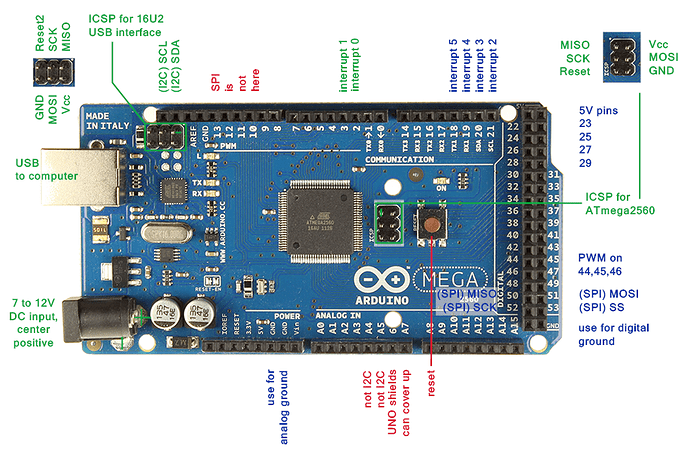
\includegraphics[width=0.65\textwidth]{resources/DomainAnalysis/HardwareComponents/arduino_mega_2560.png}%
}{%
    \fbox{\parbox{0.63\textwidth}{\centering\color{gray}\small
        [Photo pending --- save to resources/DomainAnalysis/HardwareComponents/arduino\_mega\_2560.png]}}%
}
\caption{Arduino Mega 2560 development board}
\label{fig:arduino_mega_2560}
\end{figure}

\subsubsection{Push Button}

A standard tactile momentary push button is used as the system input. The two pins on one side are internally shorted to the two pins on the other side when the button is pressed; otherwise the contacts are open. The button is wired between digital pin~7 and ground, and the internal pull-up of the ATmega2560 is enabled by configuring the pin as \texttt{INPUT\_PULLUP}. In this active-LOW configuration the pin reads HIGH when the button is idle and LOW while it is held. This avoids the need for an external pull-up resistor.

\begin{figure}[H]
\centering
\IfFileExists{resources/DomainAnalysis/HardwareComponents/pushbutton.png}{%
    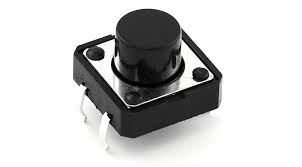
\includegraphics[width=0.45\textwidth]{resources/DomainAnalysis/HardwareComponents/pushbutton.png}%
}{%
    \fbox{\parbox{0.43\textwidth}{\centering\color{gray}\small
        [Photo pending --- save to resources/DomainAnalysis/HardwareComponents/pushbutton.png]}}%
}
\caption{Tactile push button used as the FSM input}
\label{fig:pushbutton}
\end{figure}

\subsubsection{LED and Current-Limiting Resistor}

The output device is a standard 5~mm red LED with a forward voltage of approximately 2.0~V and a maximum forward current rating of 20~mA. It is connected between digital pin~8 and ground through a 220~$\Omega$ current-limiting resistor. Applying Ohm's law for the 5~V GPIO output gives a forward current of $(5\,\mathrm{V} - 2\,\mathrm{V}) / 220\,\Omega \approx 13.6\,\mathrm{mA}$, which is comfortably below both the LED rating and the per-pin limit of the ATmega2560.

\begin{figure}[H]
\centering
\IfFileExists{resources/DomainAnalysis/HardwareComponents/led.png}{%
    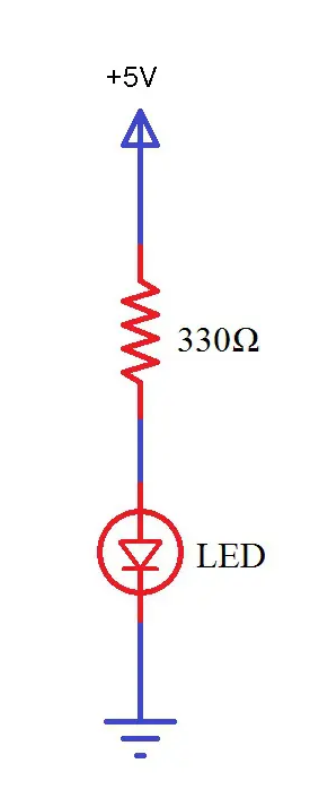
\includegraphics[width=0.18\textwidth]{resources/DomainAnalysis/HardwareComponents/led.png}%
}{%
    \fbox{\parbox{0.16\textwidth}{\centering\color{gray}\small
        [Photo pending --- save to resources/DomainAnalysis/HardwareComponents/led.png]}}%
}
\caption{Red LED used as the FSM Moore output}
\label{fig:led_component}
\end{figure}

\subsubsection{Breadboard and Jumper Wires}

A solderless breadboard provides the physical prototyping platform; jumper wires connect the Arduino pins to the button and to the resistor-LED branch. No additional hardware is required.

\subsection{Software Components}

\subsubsection{PlatformIO}

PlatformIO is the build, dependency, and tooling layer used for this project. It manages the AVR toolchain, links the Arduino framework, exposes per-environment build flags (\texttt{-DLAB6\_1} selects the Lab 6.1 entry point), and orchestrates the upload and monitor steps. The \texttt{platformio.ini} file declares an \texttt{[env:lab6\_1]} environment that compiles only the Lab 6.1 sources together with the shared libraries under \texttt{labs/lib/}, ensuring that the previous labs remain runnable from the same project tree.

\begin{figure}[H]
\centering
\IfFileExists{resources/DomainAnalysis/SoftwareComponents/platformio.png}{%
    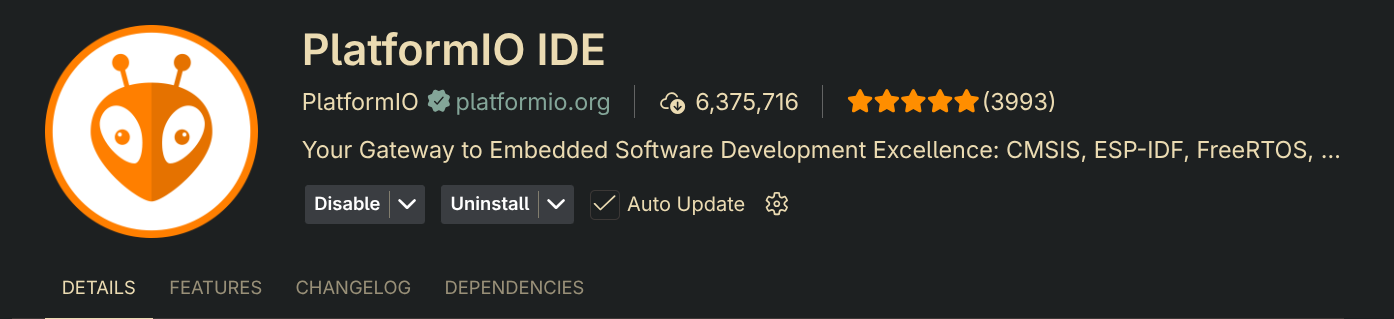
\includegraphics[width=0.75\textwidth]{resources/DomainAnalysis/SoftwareComponents/platformio.png}%
}{%
    \fbox{\parbox{0.73\textwidth}{\centering\color{gray}\small
        [Screenshot pending --- save to resources/DomainAnalysis/SoftwareComponents/platformio.png]}}%
}
\caption{PlatformIO IDE in VS Code}
\label{fig:platformio}
\end{figure}

\subsubsection{Wokwi}

Wokwi is a circuit simulator that runs Arduino firmware against a virtual board, with virtual peripherals such as buttons, LEDs, resistors, and serial terminals. It integrates with VS Code through the official Wokwi extension, which reads the lab's \texttt{wokwi.toml} pointing to the compiled firmware and the \texttt{diagram.json} describing the circuit. Wokwi is used here to validate the FSM transitions, the debounce logic, and the STDIO output without requiring physical hardware to be connected.

\begin{figure}[H]
\centering
\IfFileExists{resources/DomainAnalysis/SoftwareComponents/wokwi.png}{%
    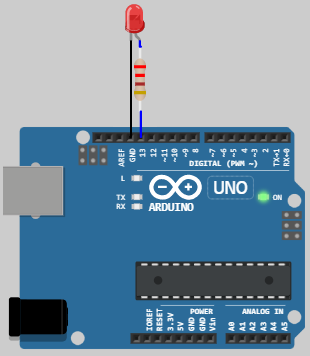
\includegraphics[width=0.75\textwidth]{resources/DomainAnalysis/SoftwareComponents/wokwi.png}%
}{%
    \fbox{\parbox{0.73\textwidth}{\centering\color{gray}\small
        [Screenshot pending --- save to resources/DomainAnalysis/SoftwareComponents/wokwi.png]}}%
}
\caption{Wokwi simulator running the Lab 6.1 circuit}
\label{fig:wokwi}
\end{figure}

\subsection{System Architecture and Justification}

The application follows the same layered architecture used throughout the course, with the FSM placed in the service layer. The Application Layer (APP) is the lab entry point \texttt{lab6\_1\_main.cpp}, whose only responsibility is to wire the drivers and the FSM together and to translate state changes into STDIO output. The Service Layer (SRV) hosts \texttt{ButtonLedFsm}, the hardware-independent Moore automaton; it knows nothing about pins or peripherals and could equally well drive a relay, an LCD line, or a remote endpoint. The ECU Abstraction Layer (ECAL) hosts \texttt{StdioSerial}, which redirects \texttt{stdout} onto UART0 so that the application can use \texttt{printf}. The Microcontroller Abstraction Layer (MCAL) provides two device drivers: \texttt{Button}, which encapsulates pin configuration, digital reads, and the debounce state machine, and \texttt{Led}, which encapsulates the digital output. The Hardware (HW) layer is the ATmega2560 peripheral set itself: GPIO ports B and H for the LED and button respectively, and USART0 for serial communication.

This decomposition is justified by two concerns. First, the lab manual explicitly requires the FSM logic to be separated from input/output drivers ("Separarea logicii FSM într-un modul software dedicat"), so that the state machine can be developed and tested independently. Second, the project rule that no \texttt{digitalRead}/\texttt{digitalWrite}/\texttt{Serial} call may appear outside \texttt{labs/lib/} forces every hardware-related operation into a clearly named driver module, which keeps the lab entry point short and readable.

\subsection{Case Study --- Real-World Applicability}

The Button-LED FSM is a minimal example, but the underlying pattern --- "a debounced discrete input drives a finite-state controller that produces a stable physical output" --- is one of the most pervasive idioms in embedded systems. Power buttons of consumer electronics implement exactly this two-state machine, sometimes with a long-press transition added for a third state ("force off"). Industrial pendant panels use FSMs to gate motor activation behind operator confirmation. Smart home wall switches that toggle relays through a single push button rely on the same logic, sometimes augmented with a network-driven external transition. In automotive electronics, many cabin functions (cruise-control engagement, hazard lights, parking brakes) are modelled as finite-state machines whose discrete inputs are debounced and whose outputs are stable Moore signals. The discipline of expressing such behaviour as a state table rather than as ad-hoc \texttt{if/else} branches is what allows these systems to be certified, formally verified, and safely extended over their long service lifetimes.
